\documentclass[12pt]{article}

\usepackage[english]{babel}
\usepackage[utf8x]{inputenc}
\usepackage{amsmath}
\usepackage{graphicx}
\usepackage[colorinlistoftodos]{todonotes}
\usepackage{listings}
\usepackage{glossaries}
\usepackage{placeins}
\usepackage{fixltx2e}
\usepackage{scrpage2}
\usepackage{scrtime}

\clearscrheadfoot
\pagestyle{scrheadings}
\usepackage[
top    = 1cm,
bottom = 1cm,
left   = 1cm,
right  = 1cm]{geometry}
\setcounter{secnumdepth}{4}

\author{RoboNav}
\date{\today}


\begin{document}


\begin{titlepage}
\begin{center}
% Oberer Teil der Titelseite:

%NEEDS TO BE OUT COMMENTED sometimes
%\includegraphics[width=1.0\textwidth]{../../pictures/robonavlogo}\\  
\rule{1.0\textwidth}{1mm}
{ \huge \bfseries \\[0.4cm]  \huge Einladung zum Schulball \\ \LARGE 'Der Hutmacher Ball' \\[0.4cm] }

\rule{1.0\textwidth}{1mm}
\vspace{0.5cm}

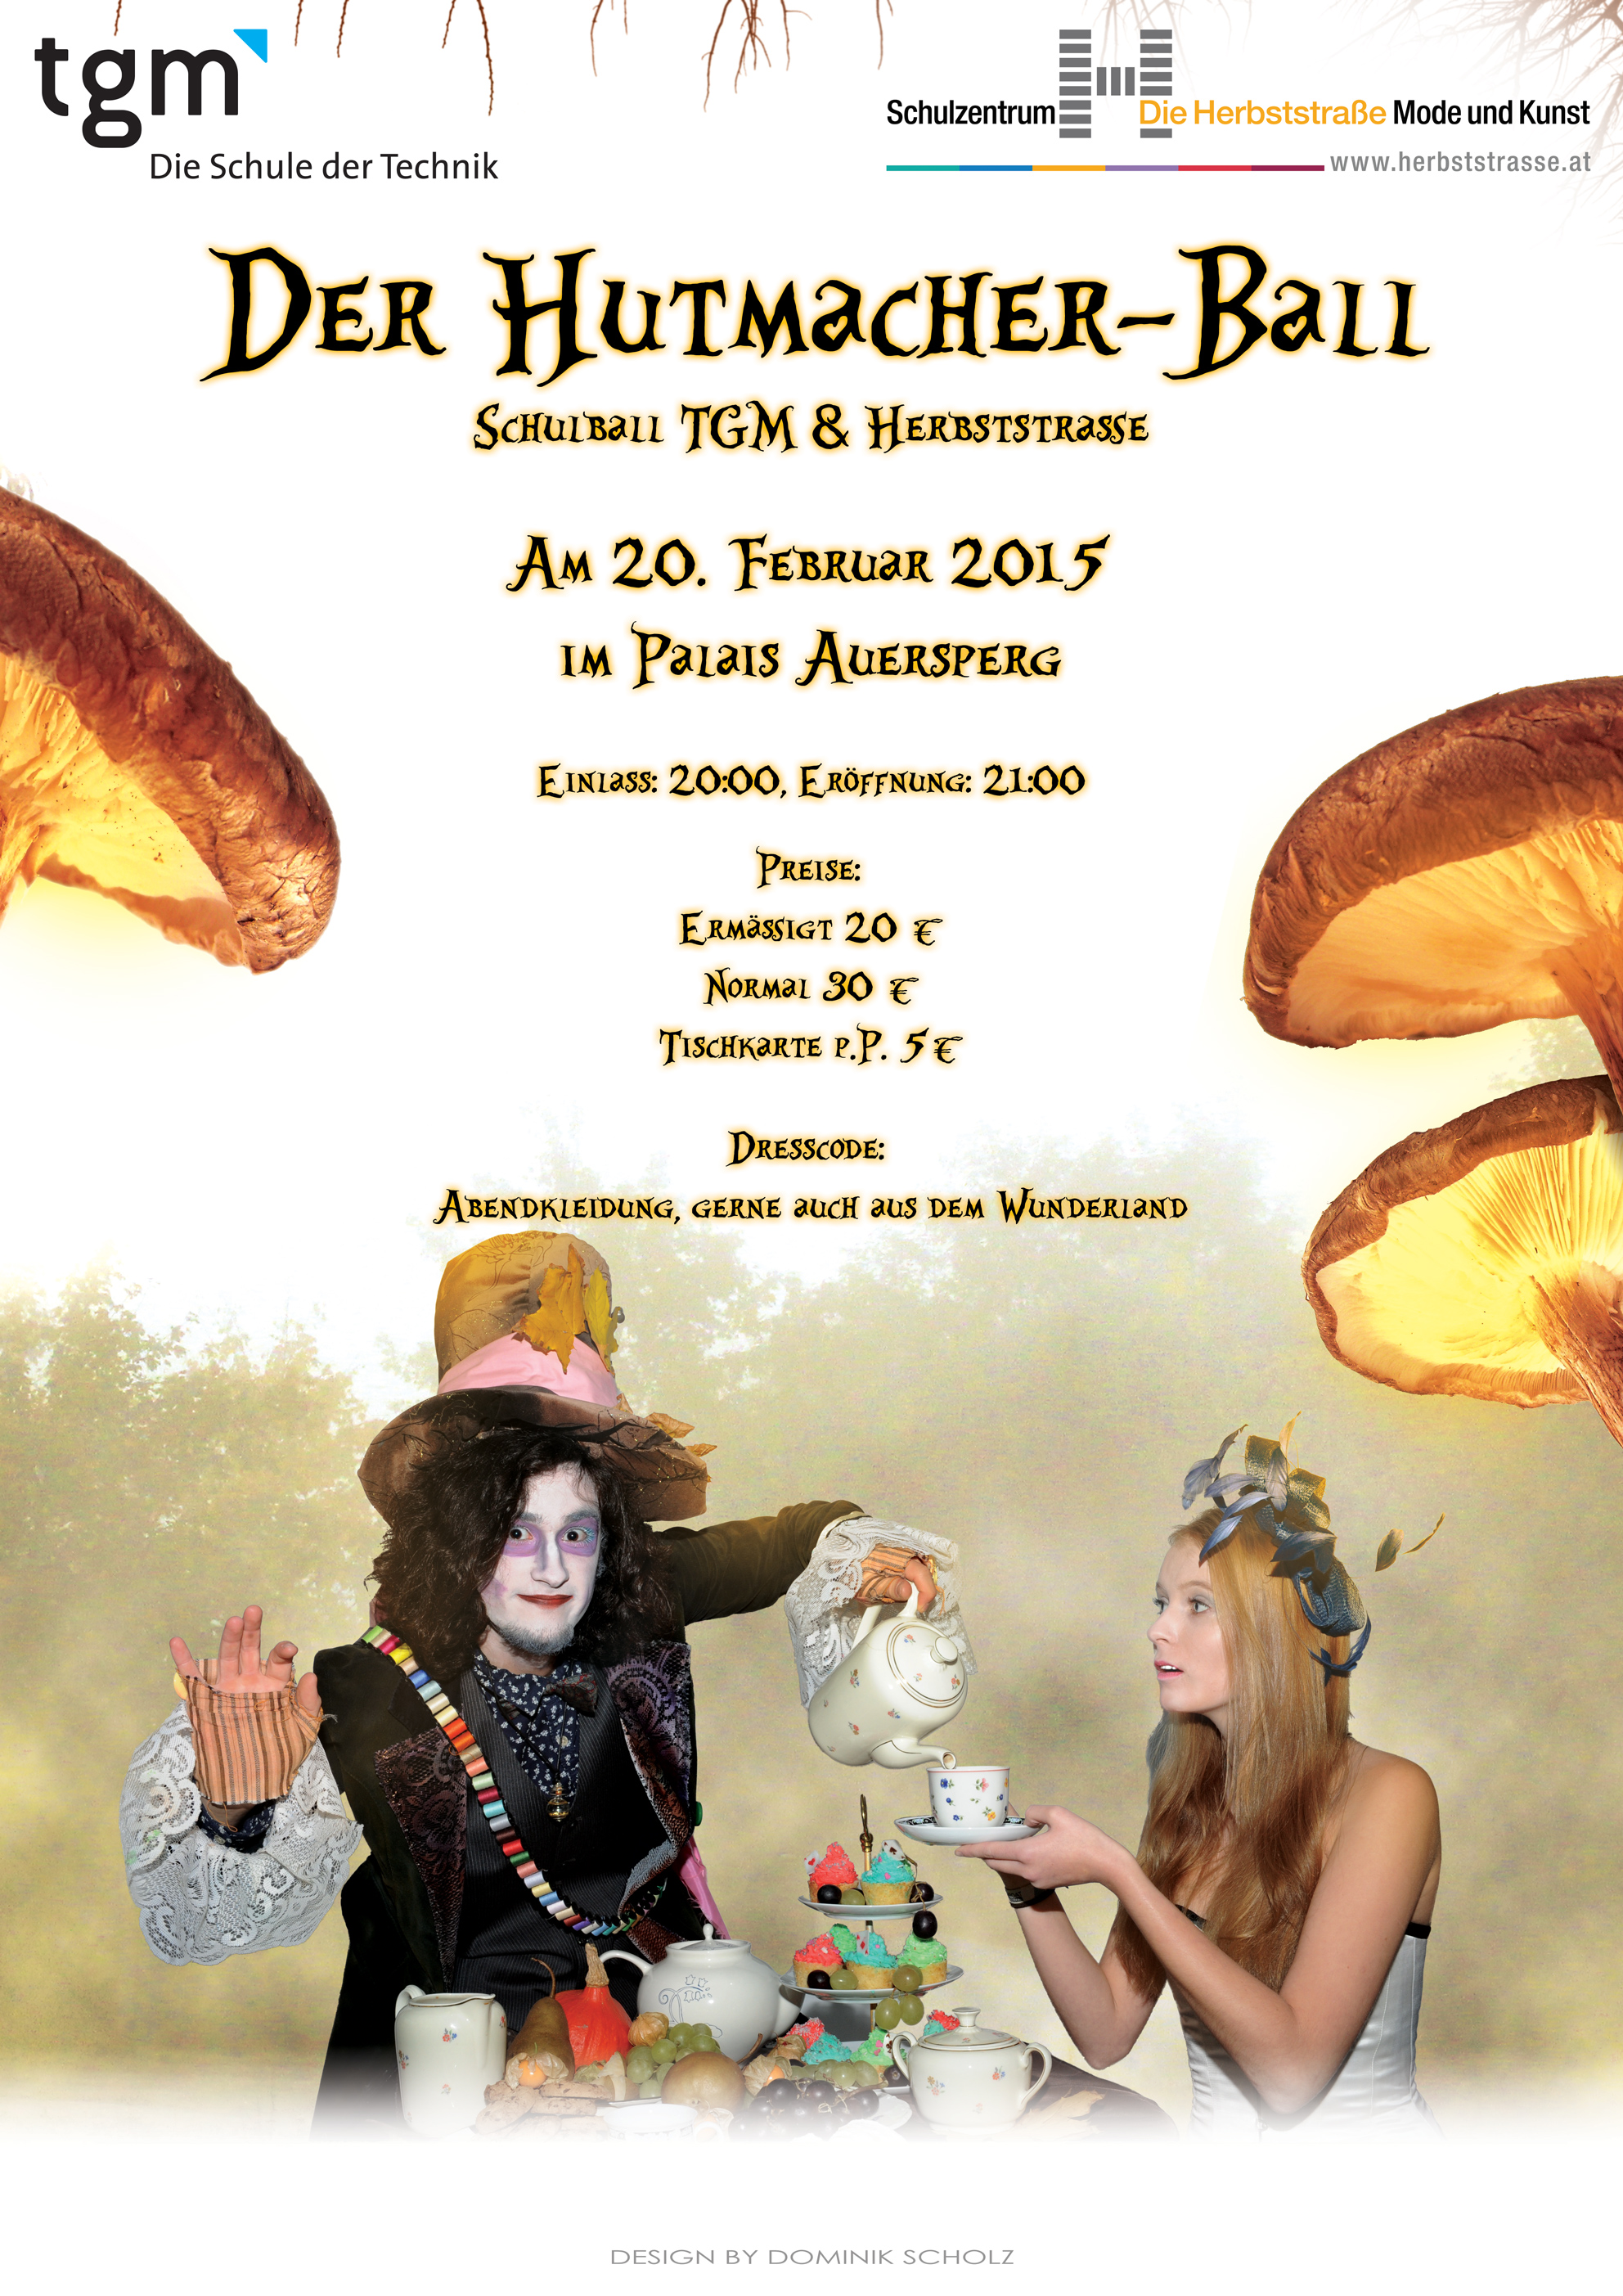
\includegraphics[width=0.7\textwidth]{ballplakatNEW}\\  

\small TGM - HTBLuVA Wien XX \\ [1.5cm]

\end{center}
\end{titlepage} 
\begin{center}
\textbf{Liebe Schüler und Schülerinnen!}
\end{center}
\vspace{0.6cm}
Das Schulballkomite möchte euch herzlichst zum diesjährigen Schulball einladen: \\
Er findet am 20. Februar ab 20:00 (Eröffnung 21:00) im Palais Auersperg statt.\\
\\ \\
\textbf{Eintrittskarten} \\
Ab dem 15.Dezember startet der Kartenverkauf beim Verband der Technologen und Technologinnen (im 1.Stock). Dort gibt es auch die Möglichkeit, Tischkarten zu kaufen. Für AbendschülerInnen wird ein gesonderter Kartenverkauf stattfinden. Die Termine hierfuer sind am Donnerstag dem 18. Dezember, am Donnerstag dem 8. Jänner und am Mittwoch dem 28.Jänner jeweils von 16:00-17:00 und 18:00-19:00 im 9. Stock. Sollten diese Termine nicht günstig sein, schreibt bitte ein Mail an hannah.siegel@student.tgm.ac.at.
\\ \\
\textbf{Eintanzen} \\
Wir suchen wieder insbesondere Herren, aber auch Paare und Damen, welche den Schulball eröffnen wollen. \\
Die Formulare für die Anmeldung findet ihr anbei. Die Termine sind vorraussichtlich: \\
Mittwoch, 11.2.2015 - 17 bis 19 Uhr \\ 
Donnerstag, 12.2.2015 - 17 bis 19 Uhr \\
Donnerstag, 19.2.2015 - 17 bis 19 Uhr \\
Generalprobe am 20.2.2015 im Ballsaal ab 18 Uhr \\ \\
\textbf{Schulball App} \\
Es wird dieses Jahr erstmalig ein Schulball App für Android geben, welches am TGM entwicklet wurde. Genaue Informationen hierzu werdet ihr vorrausichtlich Anfang Februar per Email bekommen.
\\ \\
\textbf{Crash Kurs in Klassischem Tanz} \\
Es wird in Kooperation mit der Herbststrasse ein Tanz-Crash Kurs angeboten. Dieser ist gratis und es werden die Grundlagen der Standardtänze gelernt. \\
Solltet ihr Interesse haben hierbei teilzunehmen, meldet euch bitte über die beiliegenden Formulare an. Mittwoch, 28.1.2015 - 14 bis 15 Uhr \\ 
Mittwoch, 04.2.2015 - 14 bis 15 Uhr \\ 
Mittwoch, 11.2.2015 - 14 bis 15 Uhr \\
Donnerstag, 18.2.2015 - 14 bis 15 Uhr 
\\ \\
\textbf{Rauchen} \\
Vorraussichtlich ist das Rauchen in den Ballsälen nicht mehr erlaubt.
Das Schulballkomitee ist sich diesem Problem bewusst und es wird nach einer Outdoor-Lösung für die gesamte Ballnacht gesucht. Dies ist allerdings nur unter der Vorraussetzung möglich, dass sich alle Personen die jenen Bereich in Anspruch nehmen wollen, nach zehn Uhr an die vorgeschriebene Zimmerlautstärke halten.  Andernfalls ist der Veranstalter auf Grund der Lärmbelästigung gegenüber den Anrainern gezwungen den Raucherbereich für den Rest des Balles ausnahmslos zu schließen.\\ \\
\textbf{Vorraussichtliche(!) Angebote} \\
Mitternachtseinlage, Mitternachtsquadrille, After Show Party, Frühstückssackerl, Polaroid Kameras, u.v.m
\\ \\
Bei Fragen wendet euch bitte an Hannah Siegel (hannah.siegel@student.tgm.ac.at)

\end{document}
